\documentclass{article}
\usepackage[utf8]{inputenc}
\usepackage[a3paper, margin=2in]{geometry}
\usepackage{yquant}
\usepackage{graphicx}
\usepackage{float}
\usepackage{tikz}
\usepackage{amsmath}
\usetikzlibrary{fit, quotes, calc}
\usetikzlibrary{shapes,arrows,fit,calc,positioning,automata}
\usepackage{braket}
\usepackage{rotating}
\usetikzlibrary{external}
\tikzexternalize[prefix=tikz/,optimize command away=\includepdf]

\begin{document}
\tikzset{XOR/.style={draw,circle,append after command={
        [shorten >=\pgflinewidth, shorten <=\pgflinewidth,]
        (\tikzlastnode.north) edge (\tikzlastnode.south)
        (\tikzlastnode.east) edge (\tikzlastnode.west)
        }
    }
}


% QNN
\begin{center}
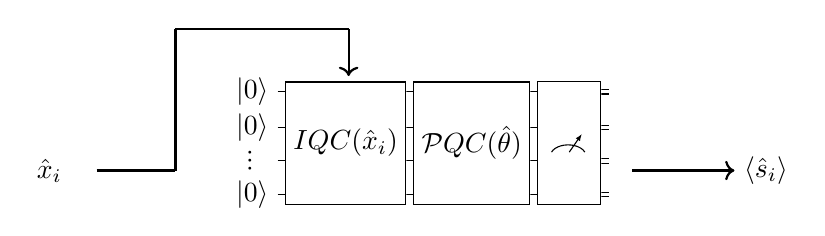
\begin{tikzpicture}[
roundnode/.style={circle, draw=red!60, fill=red!5, very thick, minimum size=4mm}
]

\begin{yquant}
    [name=loc0]
    qubit {$\ket0$} q0[1];
    [name=loc1]
    qubit {$\ket0$} q1[1];
    [name=loc2]
    qubit {\hspace{1mm} \begin{turn}{90} ... \end{turn} \hspace{1mm}} q2[1];
    [name=loc3]
    qubit {$\ket0$} q3[1];

 
    box {$IQC(\hat{x}_{i})$} (q0, q1, q2, q3);
    box {$\mathcal PQC(\hat{\theta})$} (q0, q1, q2, q3);

    measure (q0, q1, q2, q3);
  \end{yquant}


% draw arrow
\draw [thick, -] ($(loc0)+(-2,-1)$) -- ($(loc0)+(-1,-1)$);
\draw [thick, -] ($(loc0)+(-1,-1)$) -- ($(loc0)+(-1,0.8)$);
\draw [thick, -] ($(loc0)+(-1,0.8)$) -- ($(loc0)+(1.2,0.8)$);
\draw [thick, ->] ($(loc0)+(1.2,0.8)$) -- ($(loc0)+(1.2,0.2)$);
\node[] at ($(loc0)+(-2.6,-1)$) {$\hat{x}_i$};


% draw arrow
\draw [thick, ->] ($(loc0)+(4.8,-1)$) -- ($(loc0)+(6.1,-1)$);
\node[] at ($(loc0)+(6.5,-1)$) {$\left\langle  \hat{s}_i \right\rangle$};

\end{tikzpicture}
\end{center}



% pipeline
\begin{center}
\begin{tikzpicture}[
node_small/.style={rectangle, draw=black!60, fill=none, thick, dashed, minimum width=1cm,minimum height=.5cm},
node_big/.style={rectangle, draw=red!60, fill=red!5, very thick, minimum width=2.5cm,minimum height=1.5cm, rounded corners=2mm},
node_bigger/.style={rectangle, draw=red!60, fill=red!5, very thick, minimum width=3.5cm,minimum height=1.5cm, rounded corners=2mm},
]

% Define blocks
\node[node_small] (MLP) {MLP};
\node (XOR-aa)[XOR,scale=1.2] at ($(MLP)+(1.5,0)$) {};

\node[node_big]  at ($(XOR-aa)+(2.5,-0.375)$)    (EdgeNet0) {};
\node (XOR-0)[XOR,scale=1.2] at ($(EdgeNet0)+(-0.75,-0.25)$) {};
\node[node_small] at ($(EdgeNet0)+(0.5,-0.25)$) (HNN0) {HNN};
\node[] at ($(EdgeNet0.north)+(0,0.3)$) {Edge Network};

\node[node_bigger]  at ($(EdgeNet0)+(4,0)$)    (NodeNet) {};
\node[node_small] at ($(NodeNet)+(-1,0.25)$) (dot) {$s_{jk}h_j^l$};
\node (XOR-1)[XOR,scale=1.2] at ($(NodeNet)+(0,-0.25)$) {};
\node[node_small] at ($(NodeNet)+(1.0,-0.25)$) (HNN1) {HNN};
\node[] at ($(NodeNet.north)+(0,0.3)$) {Node Network};

\node[node_big]  at ($(NodeNet)+(4,0)$)    (EdgeNet1) {};
\node (XOR-2)[XOR,scale=1.2] at ($(EdgeNet1)+(-0.75,-0.25)$) {};
\node[node_small] at ($(EdgeNet1)+(0.5,-0.25)$) (HNN2) {HNN};
\node[] at ($(EdgeNet1.north)+(0,0.3)$) {Edge Network};


\node[] at ($(MLP)+(-2.5,0)$)  {$\hat{x}^i$};
\draw[thick, ->] ($(MLP)+(-2,0)$) -- (MLP.west);
\draw[thick, ->] (MLP.east) -- (XOR-aa.west);

% Input Lines

\node[] at ($(MLP)+(-2.5,-1.5)$)  {$e_{jk}$};
\draw[thick, -] ($(MLP)+(-2,-1.5)$) -- ($(XOR-2)+(0,-0.875)$);

%e_ij lines
\draw[thick, ->] ($(XOR-0)+(0,-0.875)$) -- (XOR-0.south);
\draw[thick, ->] ($(XOR-1)+(0,-0.875)$) -- (XOR-1.south);
\draw[thick, ->] ($(XOR-2)+(0,-0.875)$) -- (XOR-2.south);

%h_i^l lines
\node[] at ($(XOR-aa.east)+(0.3,0.3)$)  {$\hat{h}_i^l$};
\draw[thick, ->] (XOR-aa.east) -- ($(dot.west)+(0,0.125)$);
\draw[thick, ->] ($(XOR-0)+(0,0.6)$) -- (XOR-0.north);

% output of dot product
\draw[thick, -] (dot.east) -- ($(dot.east)+(0.5,0)$);
\draw[thick, ->] ($(dot.east)+(0.5,0)$) -- (XOR-1.north);


% HNN output lines
\draw[thick, -] (HNN0.east) -- ($(NodeNet.west)+(-0.5,-0.25)$);
\draw[thick, -] ($(NodeNet.west)+(-0.5,-0.25)$) -- ($(dot.west)+(-0.75,-0.125)$);
\draw[thick, ->] ($(dot.west)+(-0.75,-0.125)$) -- ($(dot.west)+(0,-0.125)$);
\node[] at ($(NodeNet.west)+(-0.5,-0.6)$)  {$s_{jk} $};
\draw[thick, ->] (HNN1.east) -- (XOR-2.west);
\node[] at ($(EdgeNet1.west)+(-0.5,-0.6)$)  {$\hat{h}_i^{l+1}$};

% concat output lines
\draw[thick, ->] (XOR-0.east) -- (HNN0.west);
\draw[thick, ->] (XOR-1.east) -- (HNN1.west);
\draw[thick, ->] (XOR-2.east) -- (HNN2.west);

% feedback loop
\draw[thick, -] ($(EdgeNet1.west)+(-0.5,-0.25)$) -- ($(EdgeNet1.west)+(-0.5,1.5)$);
\draw[thick, -] ($(EdgeNet1.west)+(-0.5,1.5)$) -- ($(XOR-aa)+(0,1.125)$);
\draw[thick, ->] ($(XOR-aa)+(0,1.125)$) -- (XOR-aa.north);
\node[] at ($(NodeNet.west)+(-0.5,1.7)$)  {$n_{iter}$};

% output line
\draw[thick, ->] (HNN2.east) -- ($(HNN2.east)+(1.5,0)$) ;
\node[] at ($(HNN2.east)+(1.8,0)$)  {$y_{jk}^i$};

\end{tikzpicture}
\end{center}

\newpage

Information Encoding Circuit

\begin{center}
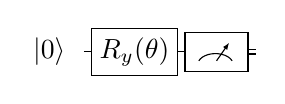
\begin{tikzpicture}[]
\begin{yquant}
    qubit {$\ket{0}$ } a[1];
    [name=inits]
    box {$R_y(\theta)$} a[0];
    measure a[0];
\end{yquant}

%\node[] at ($(inits)+(1.2,0)$) {$\ket{\Psi}_\theta$};

\end{tikzpicture}
\end{center}

\begin{center}
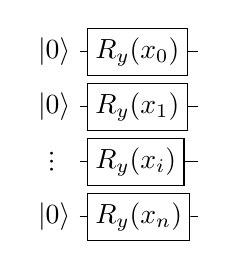
\begin{tikzpicture}

\begin{yquant}

    qubit {$\ket0$} q0[1];
    qubit {$\ket0$} q1[1];
    qubit {\hspace{1mm} \begin{turn}{90} ... \end{turn} \hspace{1mm}} q2[1];
    qubit {$\ket0$} q3[1];

    box {$R_y(x_0)$} (q0);
    box {$R_y(x_1)$} (q1);
    box {$R_y(x_i)$} (q2);
    box {$R_y(x_n)$} (q3);
 
  \end{yquant}
  \end{tikzpicture}
\end{center}

\newpage
TTN  8-qubit Circuit

\begin{center}
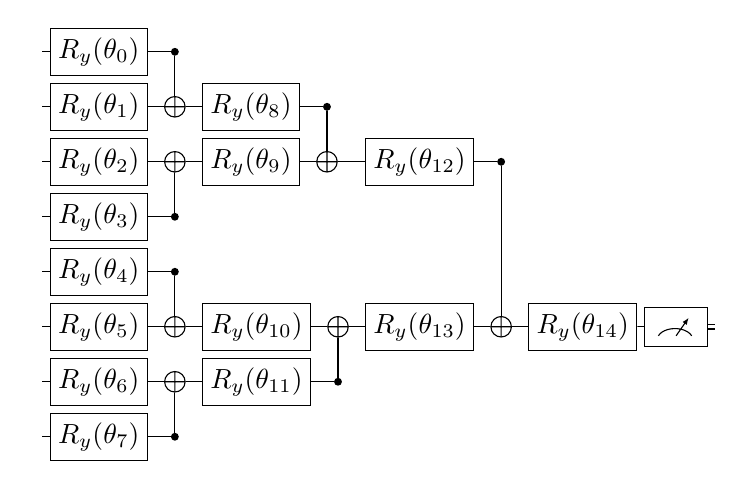
\begin{tikzpicture}
\begin{yquant}

    qubit { } a[8];

    box {$R_y(\theta_0)$} a[0];
    box {$R_y(\theta_1)$} a[1];
    cnot a[1]  |  a[0];
    discard a[0];
    box {$R_y(\theta_2)$} a[2];
    box {$R_y(\theta_3)$} a[3];
    cnot a[2]  |  a[3];
    discard a[3];
    box {$R_y(\theta_4)$} a[4];
    box {$R_y(\theta_5)$} a[5];
    cnot a[5]  |  a[4];
    discard a[4];
    box {$R_y(\theta_6)$} a[6];
    box {$R_y(\theta_7)$} a[7];
    cnot a[6]  |  a[7];
    discard a[7];
    align a;
    box {$R_y(\theta_8)$} a[1];
    box {$R_y(\theta_9)$} a[2];
    cnot a[2]  |  a[1];
    discard a[1];
    box {$R_y(\theta_{10})$} a[5];
    box {$R_y(\theta_{11})$} a[6];
    cnot a[5]  |  a[6];
    discard a[6];
    align a;
    box {$R_y(\theta_{12})$} a[2];
    box {$R_y(\theta_{13})$} a[5];
    cnot a[5]  |  a[2];
    discard a[2];
    align a;
    box {$R_y(\theta_{14})$} a[5];
    measure a[5];
  \end{yquant}
\end{tikzpicture}
\end{center}

\newpage

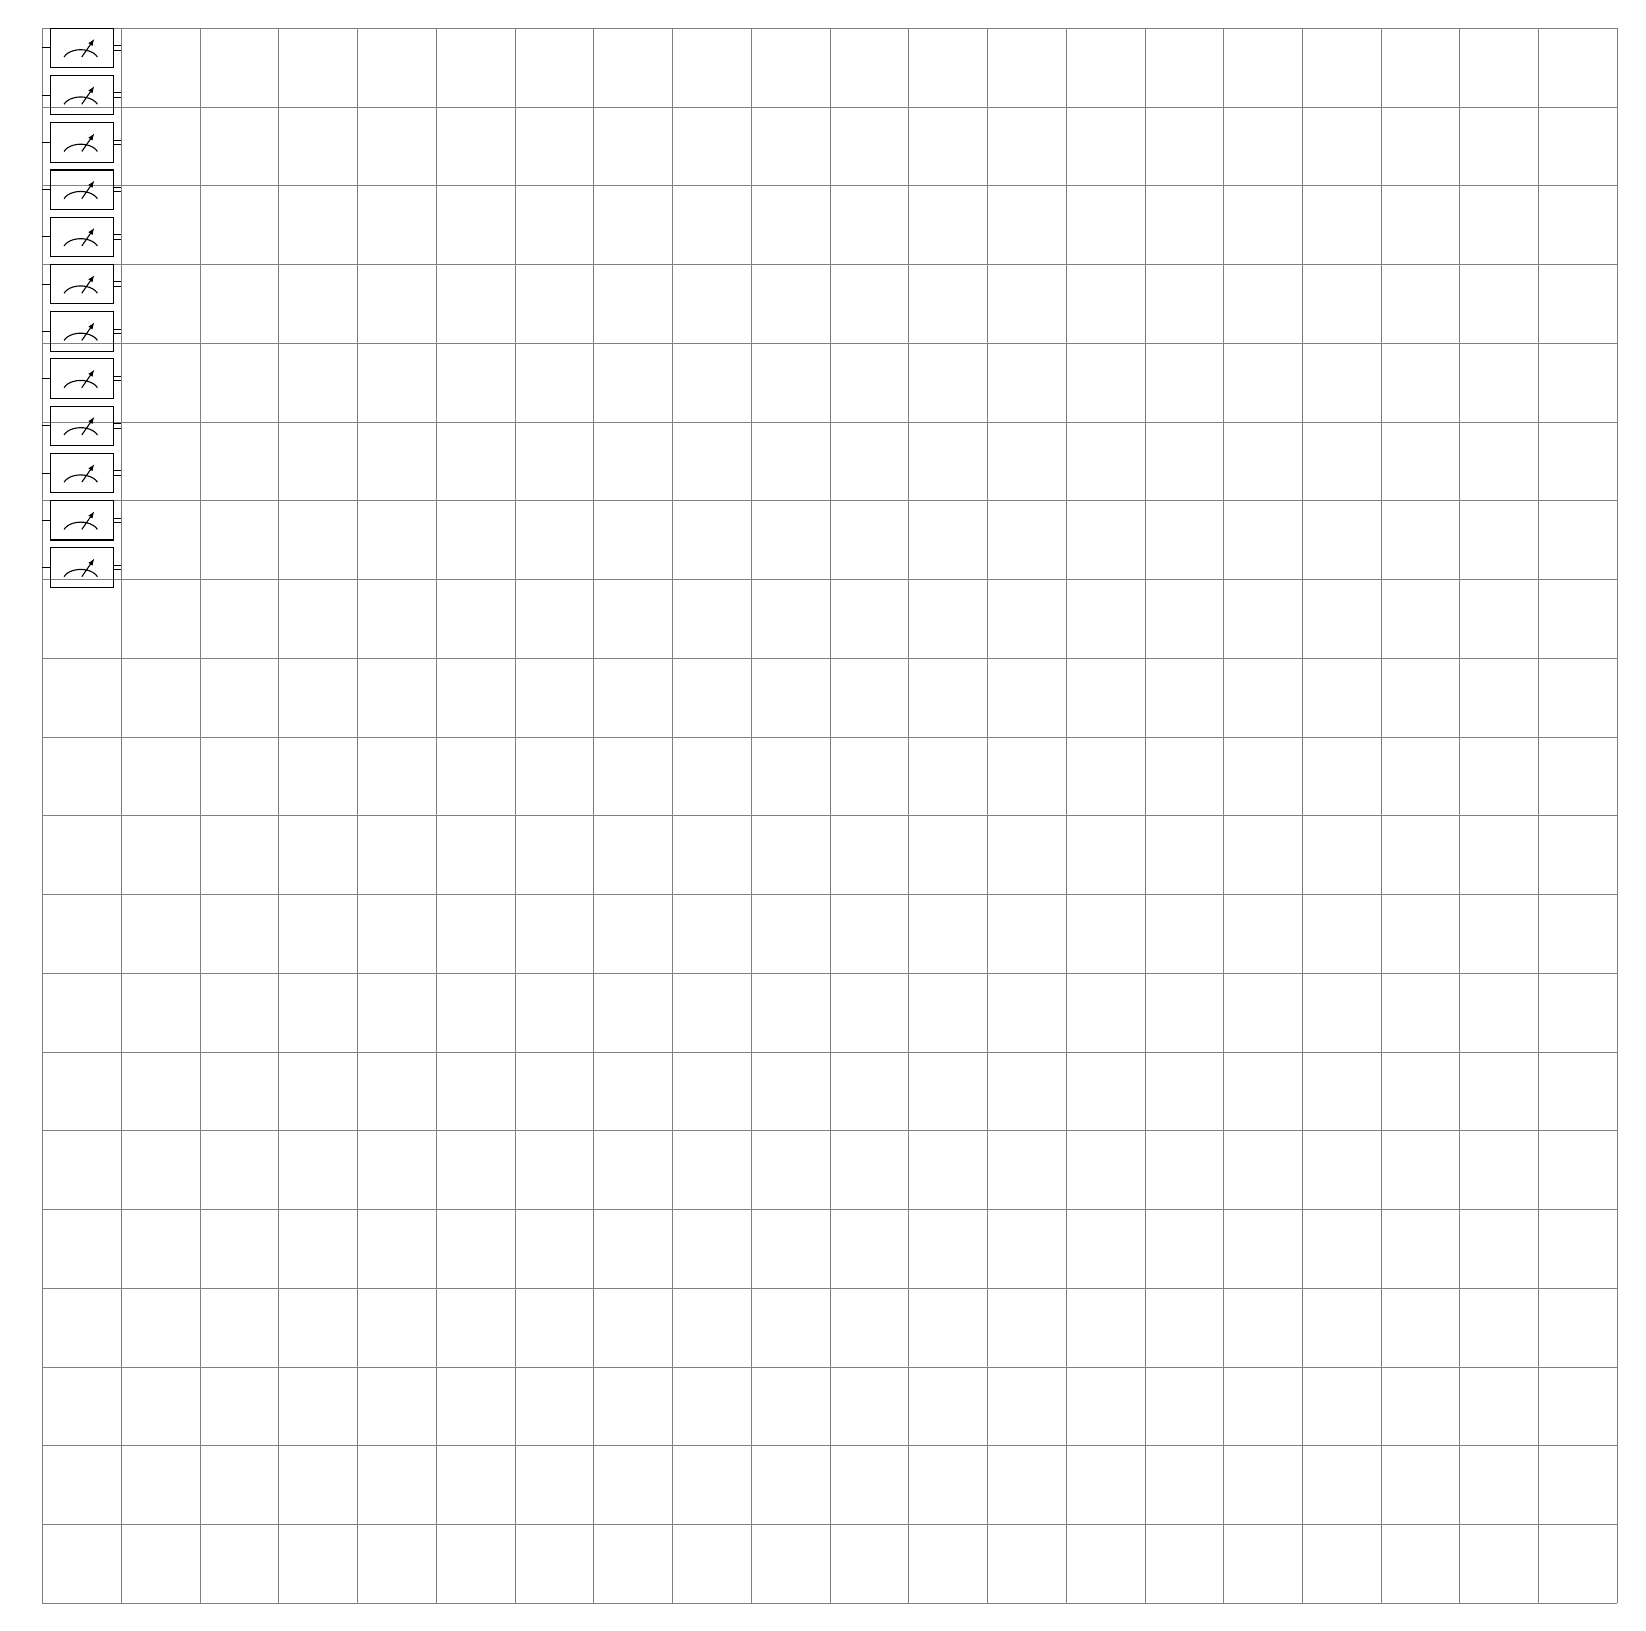
\begin{tikzpicture}
\draw[help lines] (0,0) grid(20,-20);
\begin{yquant}

    qubit { } a[12];


    %box {$R_Y(\theta_0)$} b[0];
    %box {$R_Y(\theta_1)$} b[1];
    %box {$R_Y(\theta_2)$} b[2];
    %box {$R_Y(\theta_3)$} b[3];
    %box {$R_Y(\theta_4)$} b[4];
    %box {$R_Y(\theta_5)$} b[5];
    %box {$R_Y(\theta_6)$} b[6];
    %box {$R_Y(\theta_7)$} b[7];
    %box {$R_Y(\theta_8)$} b[8];
    %box {$R_y(\theta_9)$} b[9];
    %box {$R_y(\theta_{10})$} b[10];
    %box {$R_y(\theta_{11})$} b[11];

    %cnot a[2]   |  a[3];
    %cnot b[5]   |  b[4];
    %cnot b[6]   |  b[7];
    %cnot b[9]   |  b[8]; 
    %cnot b[2] |  b[3];
     %measure a;
     measure a;

    %discard a[0];
    %discard a[4];
    %discard a[7];
    %discard a[8];
    %discard a[11];
    %align a;
   
\end{yquant}
\end{tikzpicture}


\newpage
MERA 8-qubit Circuit

\begin{center}
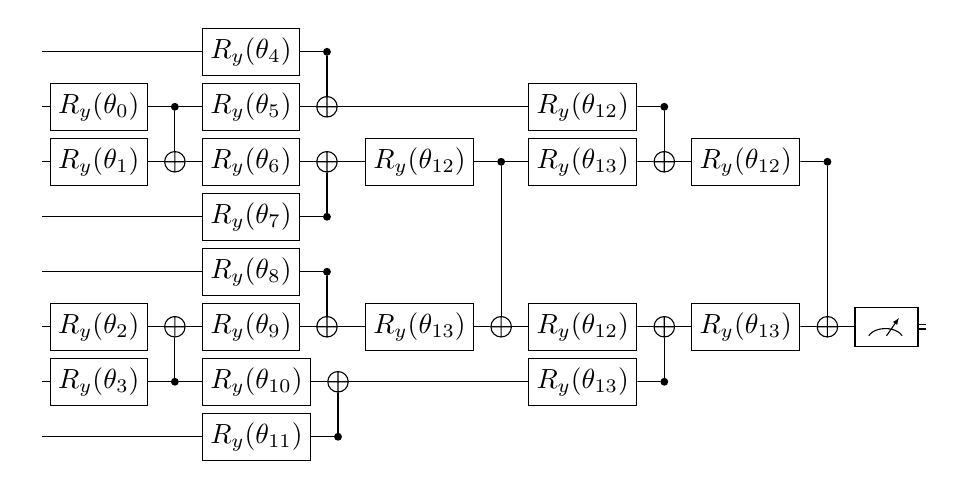
\begin{tikzpicture}
\begin{yquant}

    qubit { } a[8];
    box {$R_y(\theta_0)$} a[1];
    box {$R_y(\theta_1)$} a[2];
    cnot a[2]  |  a[1];
    box {$R_y(\theta_2)$} a[5];
    box {$R_y(\theta_3)$} a[6];
    cnot a[5]  |  a[6];
    
    align a;
    box {$R_y(\theta_4)$} a[0];
    box {$R_y(\theta_5)$} a[1];
    cnot a[1]  |  a[0];
    discard a[0];
    box {$R_y(\theta_6)$} a[2];
    box {$R_y(\theta_7)$} a[3];
    cnot a[2]  |  a[3];
    discard a[3];
    box {$R_y(\theta_8)$} a[4];
    box {$R_y(\theta_9)$} a[5];
    cnot a[5]  |  a[4];
    discard a[4];
    box {$R_y(\theta_{10})$} a[6];
    box {$R_y(\theta_{11})$} a[7];
    cnot a[6]  |  a[7];
    discard a[7];
    
    align a;
    box {$R_y(\theta_{12})$} a[2];
    box {$R_y(\theta_{13})$} a[5];
    cnot a[5]  |  a[2];

    align a;
    box {$R_y(\theta_{12})$} a[1];
    box {$R_y(\theta_{13})$} a[2];
    cnot a[2]  |  a[1];
    discard a[1];
    box {$R_y(\theta_{12})$} a[5];
    box {$R_y(\theta_{13})$} a[6];
    cnot a[5]  |  a[6];
    discard a[6];
        
    align a;
    box {$R_y(\theta_{12})$} a[2];
    box {$R_y(\theta_{13})$} a[5];
    cnot a[5]  |  a[2];
    discard a[2];
    align a;
    measure a[5];
  \end{yquant}
\end{tikzpicture}
\end{center}


MPS 8-qubit Circuit

\begin{center}
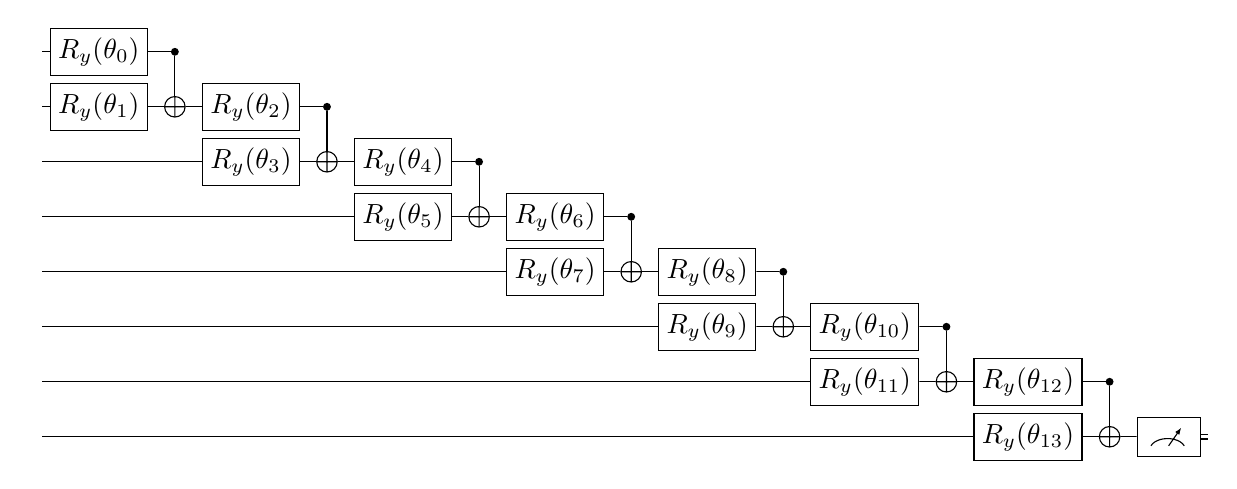
\begin{tikzpicture}
\begin{yquant}

    qubit { } a[8];

    box {$R_y(\theta_0)$} a[0];
    box {$R_y(\theta_1)$} a[1];
    cnot a[1]  |  a[0];
    discard a[0];
    align a;
    box {$R_y(\theta_2)$} a[1];
    box {$R_y(\theta_3)$} a[2];
    cnot a[2]  |  a[1];
    discard a[1];
    align a;
    box {$R_y(\theta_4)$} a[2];
    box {$R_y(\theta_5)$} a[3];
    cnot a[3]  |  a[2];
    discard a[2];
    align a;
    box {$R_y(\theta_6)$} a[3];
    box {$R_y(\theta_7)$} a[4];
    cnot a[4]  |  a[3];
    discard a[3];
    align a;
    box {$R_y(\theta_8)$} a[4];
    box {$R_y(\theta_9)$} a[5];
    cnot a[5]  |  a[4];
    discard a[4];
    align a;
    box {$R_y(\theta_{10})$} a[5];
    box {$R_y(\theta_{11})$} a[6];
    cnot a[6]  |  a[5];
    discard a[5];
    align a;
    box {$R_y(\theta_{12})$} a[6];
    box {$R_y(\theta_{13})$} a[7];
    cnot a[7]  |  a[6];
    discard a[6];
    align a;
    measure a[7];

  \end{yquant}
\end{tikzpicture}
\end{center}





\end{document}
